\subsection{Concept}
This experiment is conducted to understand two questions. One is how different pointer types have impact to runtime performance.
The other is how initialization of Vec size has impact to runtime performance. 
In this experiment, we focus on owner, reference, and additionally slice as a pointer to sequence values. 
The memory representations of these pointer types are shown in figure. 

The owner has a pointer pointing to the memory address of sequence values, length of the values, and capacity allocated to store additional values. 
The reference is a pointer that points to the owner. The slice is a pointer that points to memory address of sequence values and has value such as length of 
sequence values stored in the memory. Since they have different memory representation, an assumption is that it takes different time to access to the contents of the memory among these pointer types.

To evaluate this assumption, we use the three type of complex object.

\begin{figure}[htb]
    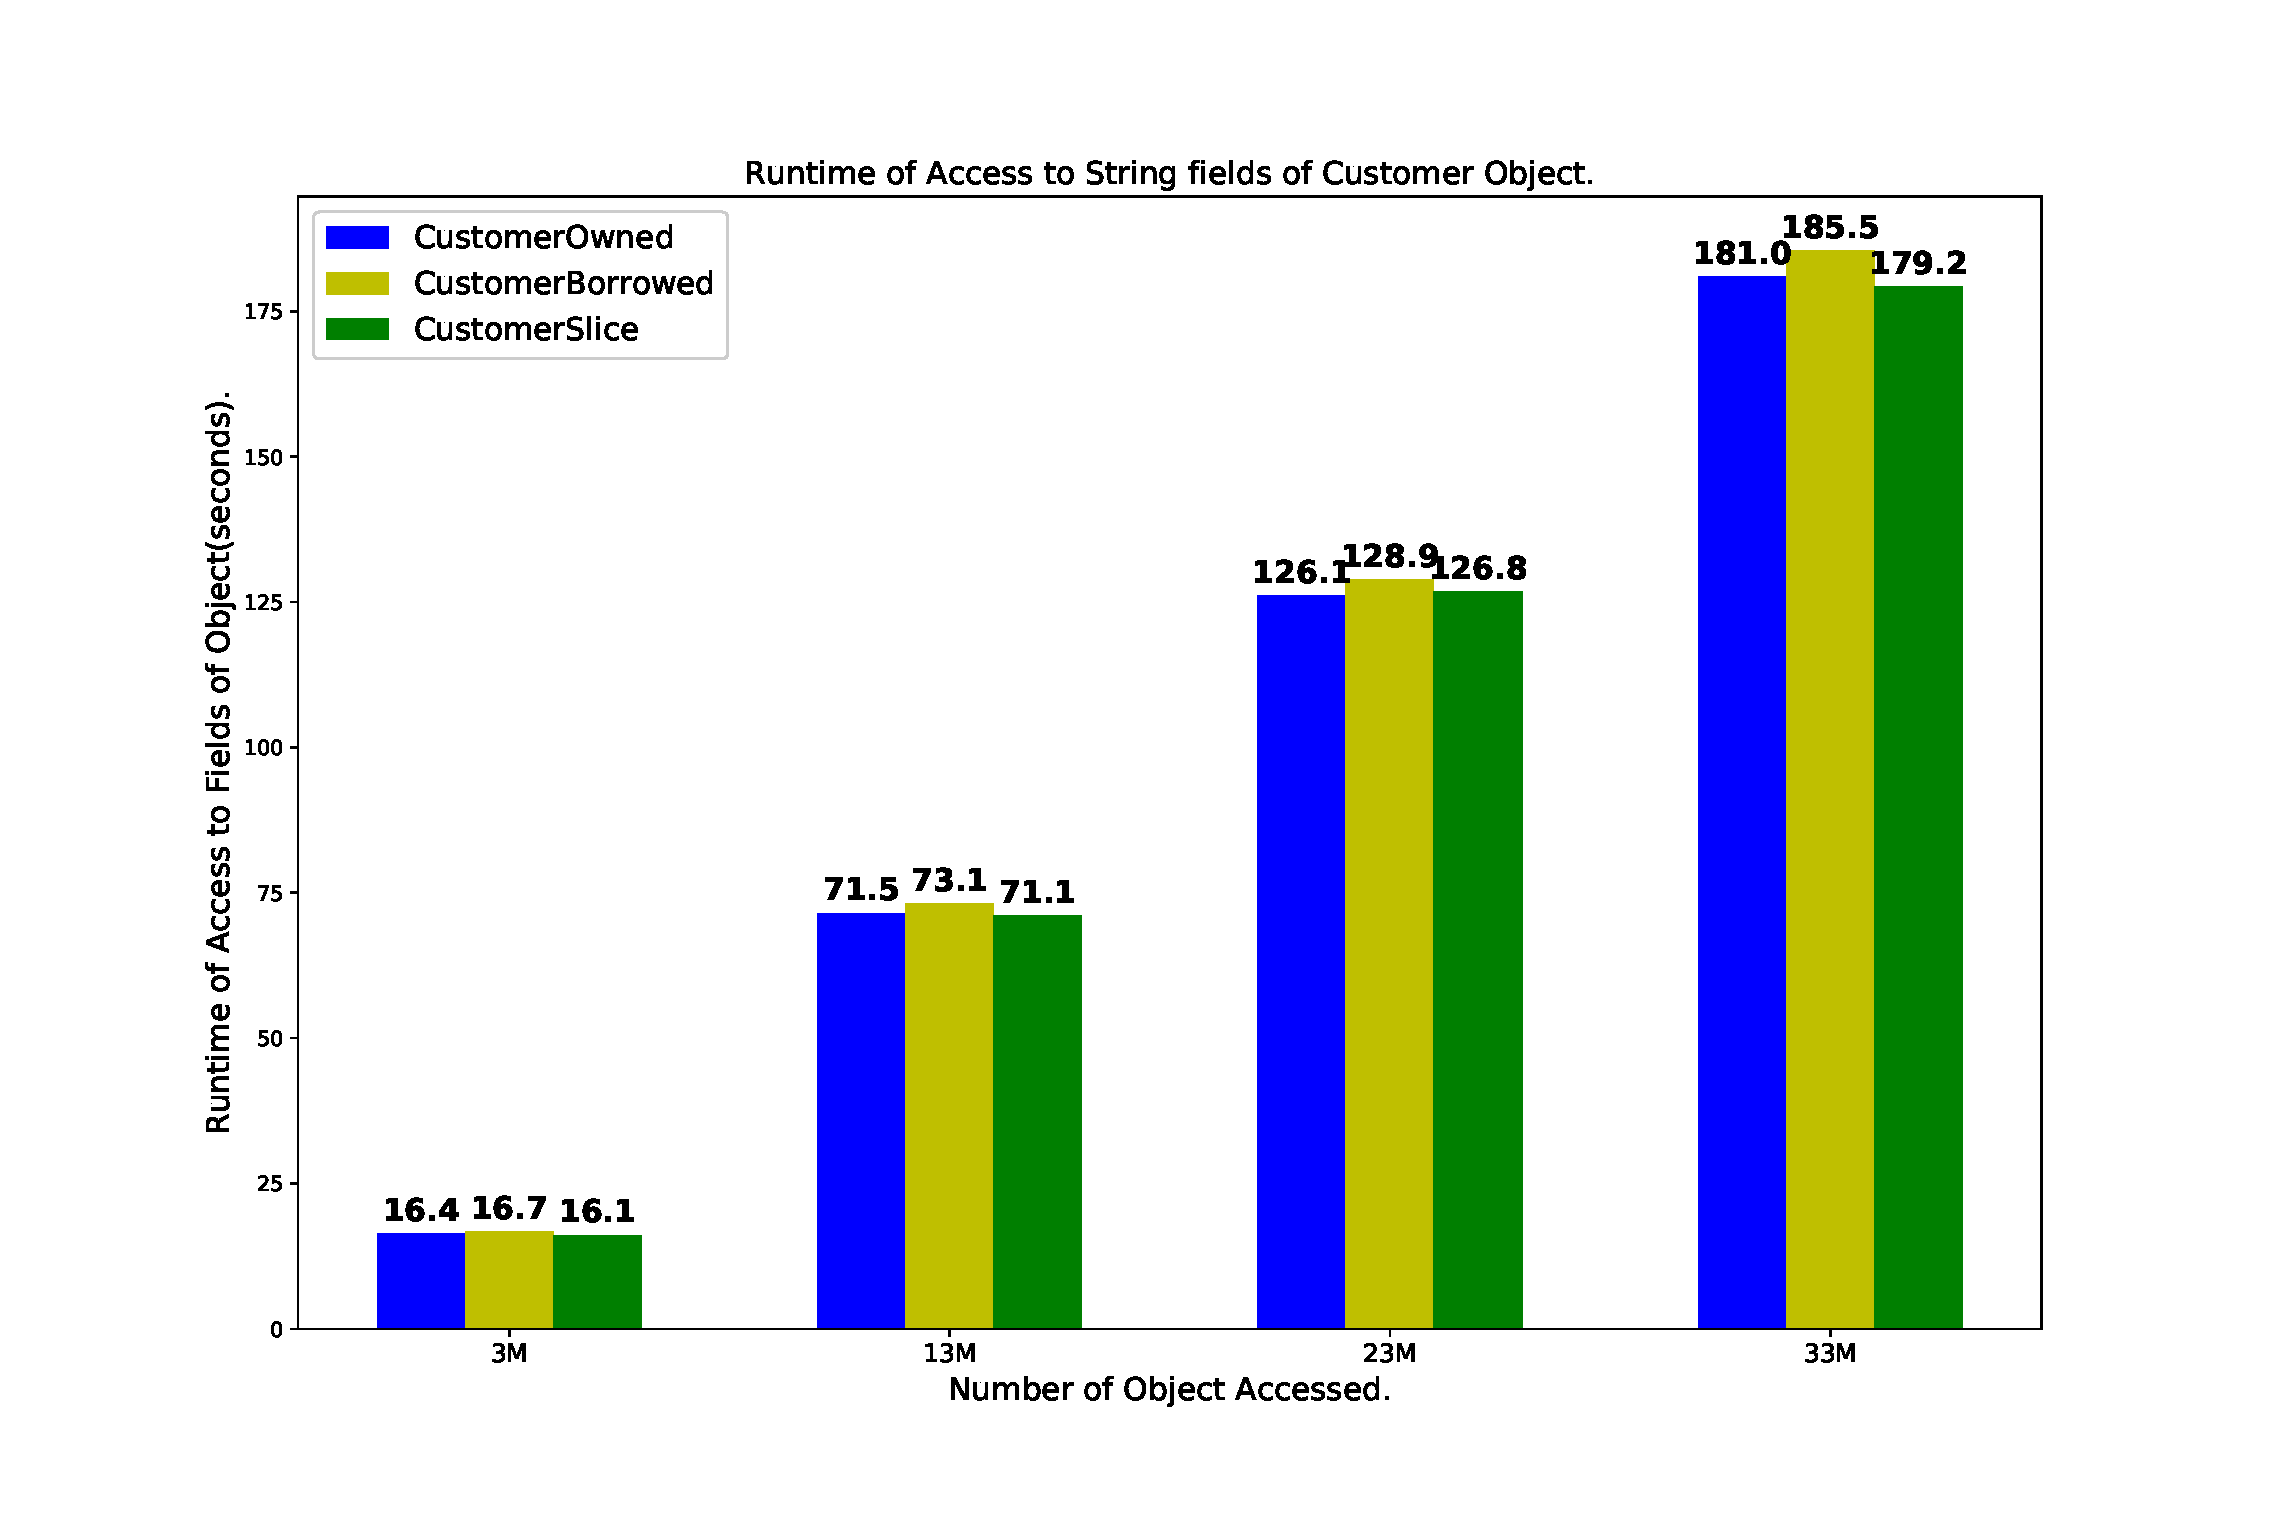
\includegraphics[width=15cm]{rust_access_different_poniter_init.eps}
    \caption{Runtime of Access to Different Pointer Types with Vec Size Initialization}
    \label{fig:rustaccessinit}
\end{figure}

\begin{figure}[htb]
    \includegraphics[width=15cm]{rust_access_different_poniter_noinit.eps}
    \caption{Runtime of Access to Different Pointer Types without Vec Size Initialization}
    \label{fig:rustaccessnoinit}
\end{figure}

\begin{figure}[htb]
    \includegraphics[width=15cm]{rust_access_init_vs_noint.eps}
    \caption{Runtime of Access to Fields of Complex Object with Initialization vs without Initialization}
    \label{fig:rustaccessnoinit}
\end{figure}


The representation of these objects are shown in Figure~\ref{fig:customer} and Figure~\ref{fig:order}. 
\begin{figure}[htb]
    \begin{minipage}[t]{0.2\linewidth}\centering
        \begin{lstlisting}
            struct CustomerOwned {
                key: i32,
                age: i32,
                num_purchase: i32,
                total_purchase: f64,
                duration_spent: f64, 
                duration_since: f64,
                zip_code: String,
                address: String,
                country: String,
                state: String,
                first_name: String,
                last_name: String,
                province: String,
                comment: String, 
                order: OrderOwned
            }
        \end{lstlisting}
      \medskip
      \centerline{(a)}
    \end{minipage}\hfill
    \begin{minipage}[t]{0.6\linewidth}\centering
        \begin{lstlisting}
            struct CustomerBorrowed<'a> {
                key: &'a i32,
                age: &'a i32,
                num_purchase: &'a i32,
                total_purchase: &'a f64,
                duration_spent: &'a f64, 
                duration_since: &'a f64,
                zip_code: &'a String,
                address: &'a String,
                country: &'a String,
                state: &'a String,
                first_name: &'a String,
                last_name: &'a String,
                province: &'a String,
                comment: &'a String, 
                order: &'a OrderBorrowed<'a>
            }
        \end{lstlisting}
      \medskip
      \centerline{(b)}
    \end{minipage}
    \begin{minipage}[t]{0.2\linewidth}\centering
        \begin{lstlisting}
            struct CustomerSlice<'a> {
                key: &'a i32,
                age: &'a i32,
                num_purchase: &'a i32,
                total_purchase: &'a f64,
                duration_spent: &'a f64, 
                duration_since: &'a f64,
                zip_code: &'a str,
                address: &'a str,
                country: &'a str, 
                state: &'a str,
                first_name: &'a str,
                last_name: &'a str,
                province: &'a str,
                comment: &'a str,
                order: &'a OrderSlice<'a>
            }
        \end{lstlisting}
      \medskip
      \centerline{(c)}
    \end{minipage}\hfill
    \caption{Representation of Customer objects Whose fields are different variable type: (a) CustomerOwned struct whose fields are all owned 
    (b) CustomerBorrowed struct whose fields are borrowed with reference (c) CustomerSlice struct whose fields are borrowed with slice for sequence value, otherwise reference}
    \label{fig:customer}
 \end{figure}

 \begin{figure}[htb]
    \begin{minipage}[t]{0.2\linewidth}\centering
        \begin{lstlisting}
            struct OrderOwned {
                order_id: i32,
                num_items: i32, 
                payment: f64,
                order_time: f64,
                title: String,
                comment: String
            } 
        \end{lstlisting}
      \medskip
      \centerline{(a)}
    \end{minipage}\hfill
    \begin{minipage}[t]{0.6\linewidth}\centering
        \begin{lstlisting}
            struct OrderBorrowed<'a> {
                order_id: &'a i32,
                num_items: &'a i32, 
                payment: &'a f64,
                order_time: &'a f64,
                title: &'a String,
                comment: &'a String
            }
        \end{lstlisting}
      \medskip
      \centerline{(b)}
    \end{minipage}
    \begin{minipage}[t]{0.2\linewidth}\centering
        \begin{lstlisting}
            struct OrderSlice<'a> {
                order_id: &'a i32,
                num_items: &'a i32, 
                payment: &'a f64,
                order_time: &'a f64,
                title: &'a str,
                comment: &'a str
            }
        \end{lstlisting}
      \medskip
      \centerline{(c)}
    \end{minipage}\hfill
    \caption{Representation of Order objects Whose fields are different variable type: (a) OrderOwned struct whose fields are all owned 
    (b) OrderBorrowed struct whose fields are borrowed with reference (c) OrderSlice struct whose fields are borrowed with slice for sequence value, otherwise reference}
    \label{fig:order}
 \end{figure}


